\documentclass[compress,t]{beamer}
\newcommand{\thou}{,\!000}
% Copyright 2004 by Till Tantau <tantau@users.sourceforge.net>.
%
% In principle, this file can be redistributed and/or modified under
% the terms of the GNU Public License, version 2.
%
% However, this file is supposed to be a template to be modified
% for your own needs. For this reason, if you use this file as a
% template and not specifically distribute it as part of a another
% package/program, I grant the extra permission to freely copy and
% modify this file as you see fit and even to delete this copyright
% notice. 

\mode<presentation> {
  \usetheme{Malmoe}
  \usecolortheme{beaver}
  \setbeamercovered{transparent}
  \setbeamertemplate{navigation symbols}{{\small\insertpagenumber}}
%{{\normalsize\insertframenumber}}
  \setbeamertemplate{footline}{%
    \leavevmode%
    \hbox{\begin{beamercolorbox}[wd=\paperwidth,ht=0.5ex,dp=1.125ex,leftskip=.3cm,rightskip=.3cm plus1fil]{title in head/foot}%
    \end{beamercolorbox}}%
    \vskip0pt%
  }
  \setbeamertemplate{headline}{% %split theme}
  \leavevmode%
    \begin{beamercolorbox}[wd=.3\paperwidth,ht=2.5ex,dp=1.125ex]{section in head/foot}%
      \insertsectionnavigationhorizontal{.3\paperwidth}{\hskip0pt plus1filll}{}%
  \end{beamercolorbox}%
  \begin{beamercolorbox}[wd=.7\paperwidth,ht=2.5ex,dp=1.125ex]{subsection in head/foot}%
    \insertsubsectionnavigationhorizontal{.7\paperwidth}{}{\hskip0pt plus1filll}%
  \end{beamercolorbox}%
  }
  %\setbeamersize{sidebar width right=2ex}
  %{\usebeamercolor{sidebar}}
  %\setbeamertemplate{sidebar canvas right}{f \insertframenumber}
  %\insertpagenumber
}

\usepackage[english]{babel}
\usepackage[latin1]{inputenc}
\usepackage{helvet}
\usepackage{xspace}
% Or whatever. Note that the encoding and the font should match. If T1
% does not look nice, try deleting the line with the fontenc.
%\usepackage[T1]{fontenc}
\usepackage[normalem]{ulem}
\usepackage{calc}
\usepackage{verbatim}
\usepackage{multirow}
\usepackage{dcolumn}
\usepackage{multimedia} 
%\usepackage{amsbsy}
\usepackage{amsmath}

\newcommand{\arxiv}[1]{\href{http://arxiv.org/abs/#1}{arXiv:#1}}
\newcommand{\etal}{\textit{et al.~}}
\newcommand{\snr}[1]{\mathbb{SN}(#1)}

%\graphicspath{{figs-slides/}{figs-techreport/}}

\newcommand{\eg}{\emph{eg}}

% commands to add more space in \itemize environments
\newcommand{\bitmorespace}{%
  \addtolength{\itemsep}{0.5ex}%
  %\addtolength{\parskip}{0.5ex}%
  %\addtolength{\parsep}{0.5ex}%
  %\addtolength{\topsep}{0.5ex}%
  \vspace{0.5ex}%
}
\newcommand{\morespace}{\addtolength{\itemsep}{1ex}}
\newcommand{\Morespace}{\addtolength{\itemsep}{1.5ex}}


\newcommand{\commentout}[1]{}


\usefonttheme[onlymath]{serif}
\usepackage{multimedia} 

\title{Unsupervised learning \& Mixture models}
\author{Dustin Lang \\ {\small McWilliams Postdoc Fellow \\ Carnegie Mellon University \\ \emph{visiting} University of Waterloo}}
\date{Local Group Astrostats \hspace*{0.5em}/\hspace*{0.5em} 2015-06-04}

\begin{document}

\begin{frame}
  \titlepage
\end{frame}

\section{Intro}

\begin{frame}{The Machine Learning Landscape}%[plain]
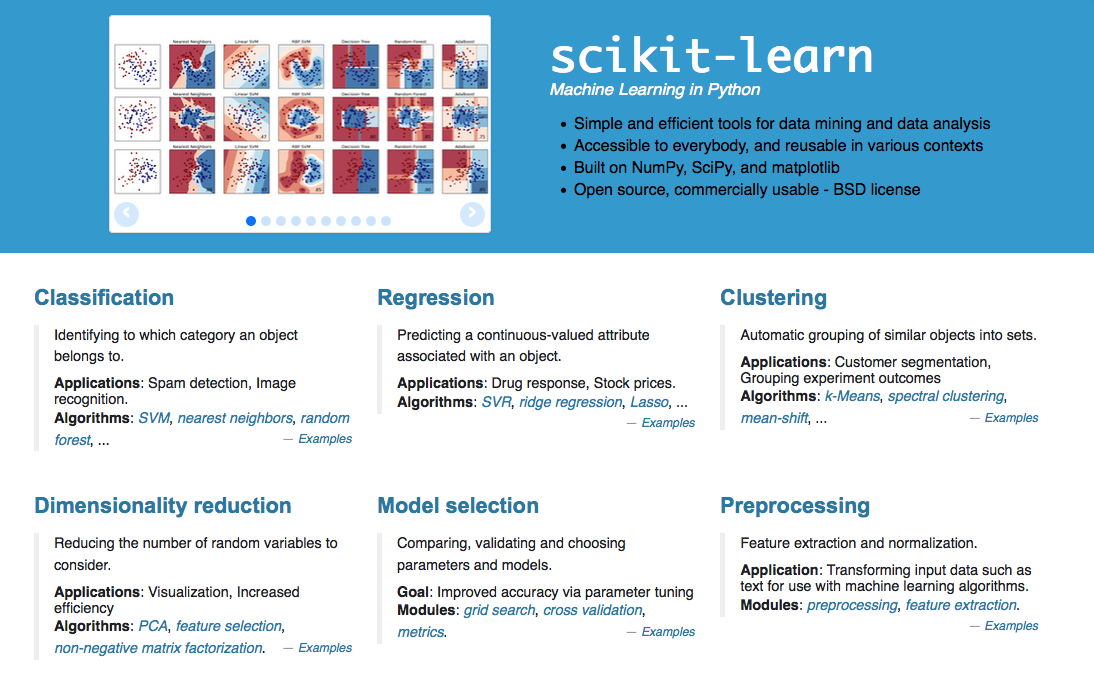
\includegraphics[width=\textwidth]{landscape}
\end{frame}

\begin{frame}{Unsupervised learning}
  \begin{itemize}
    \item \alert{No labels} / \alert{no truth}: We are not given a target value we want to reconstruct
    \item Just given the data (usually assumed: low-dimensional measurements
      with equal noise)
    \item Main task: \alert{Clustering}
  \end{itemize}

  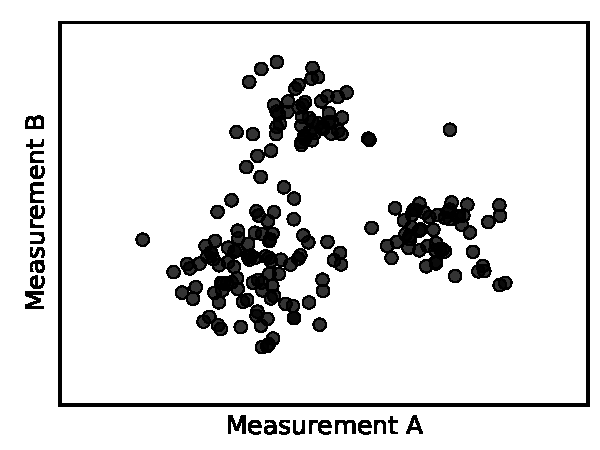
\includegraphics[width=0.4\textwidth]{ex3a}
  \hspace{1em}
  \raisebox{0.18\textheight}{$\longrightarrow$}
  \hspace{1em}
  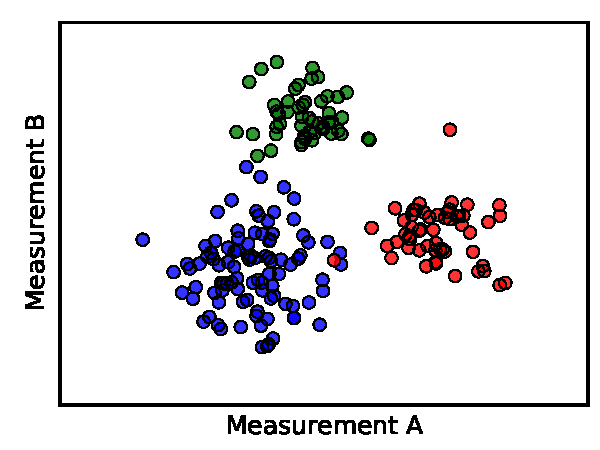
\includegraphics[width=0.4\textwidth]{ex3b}

\end{frame}

\section{K-means}

\begin{frame}{Clustering: $K$-means algorithm}
  \begin{itemize}
    \item Assume $K$ \alert{clusters}, each characterized by a \alert{centroid}
    \item Start by randomly choosing $K$ data points as centroids
    \item Iteratively:
      \begin{itemize}
      \item \alert{Assign} each data point to the \alert{nearest} cluster
      \item \alert{Compute} new cluster center based on assigned data points
      \end{itemize}
  \end{itemize}
  \begin{center}
    \only<1>{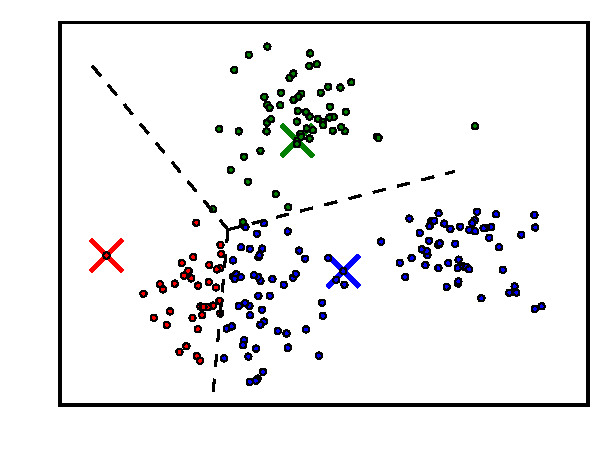
\includegraphics[width=0.7\textwidth]{kmeans-00}}%
    \only<2>{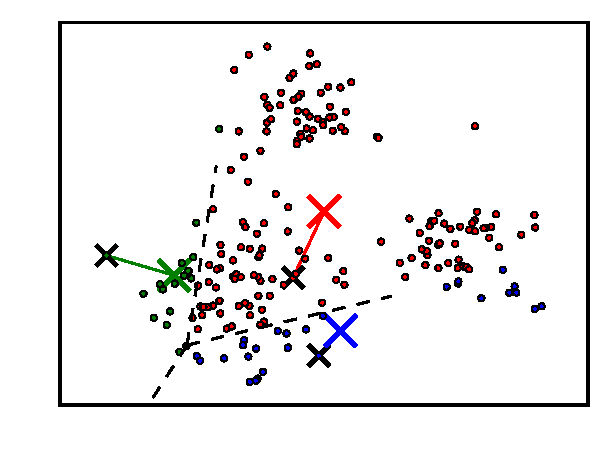
\includegraphics[width=0.7\textwidth]{kmeans-01}}%
    \only<3>{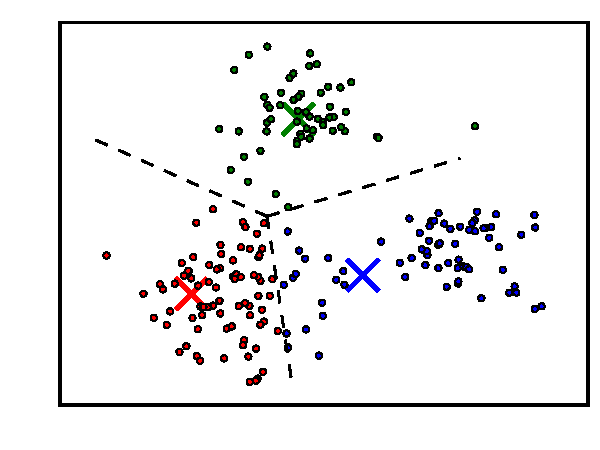
\includegraphics[width=0.7\textwidth]{kmeans-02}}%
    \only<4>{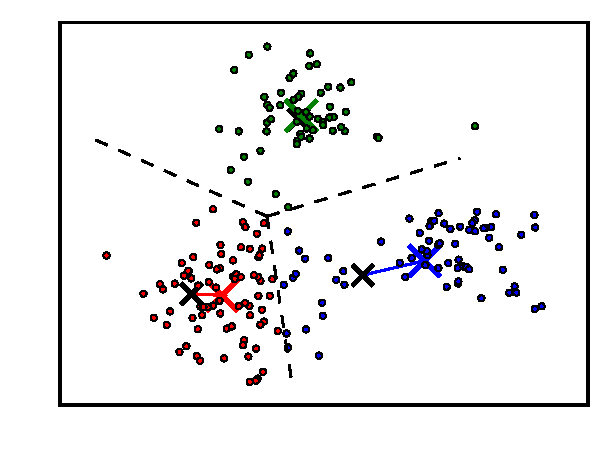
\includegraphics[width=0.7\textwidth]{kmeans-03}}%
    \only<5>{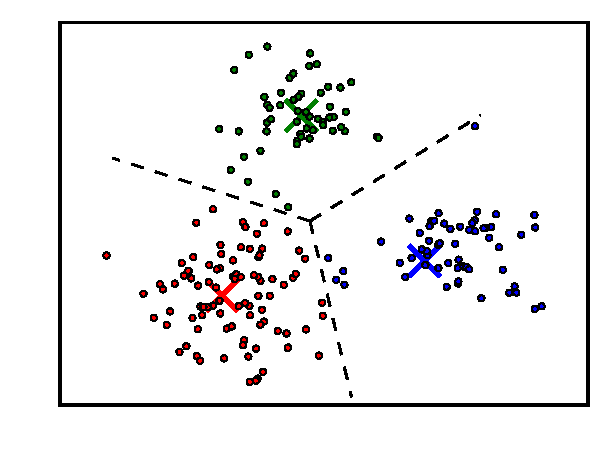
\includegraphics[width=0.7\textwidth]{kmeans-04}}%
    \only<6>{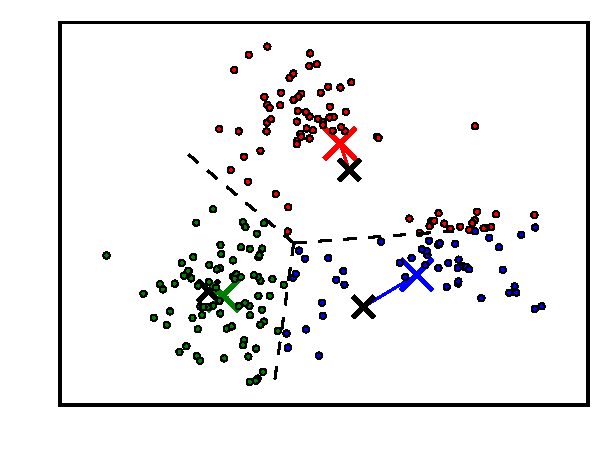
\includegraphics[width=0.7\textwidth]{kmeans-05}}%
    \only<7>{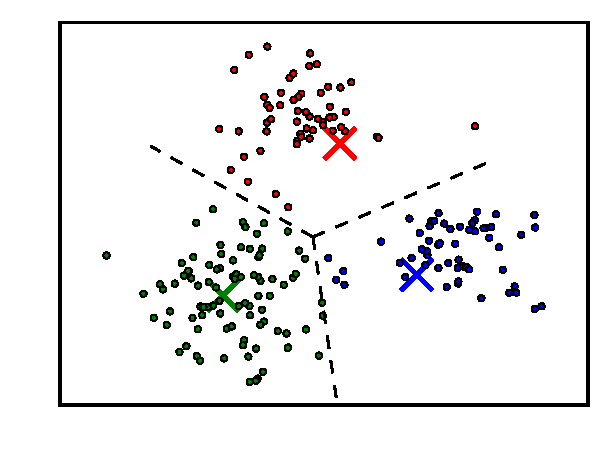
\includegraphics[width=0.7\textwidth]{kmeans-06}}%
    \only<8>{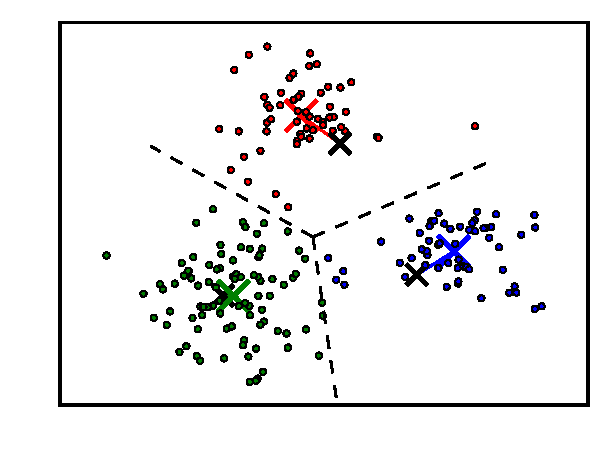
\includegraphics[width=0.7\textwidth]{kmeans-07}}%
    \only<9>{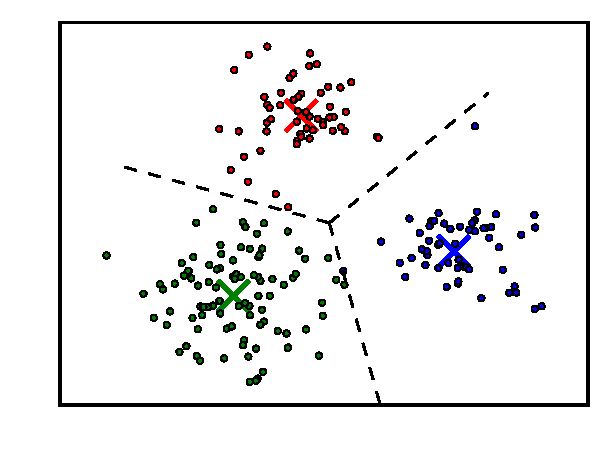
\includegraphics[width=0.7\textwidth]{kmeans-08}}%
    \only<10>{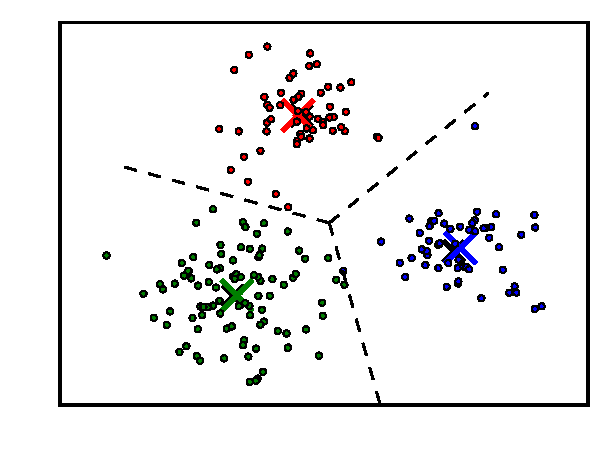
\includegraphics[width=0.7\textwidth]{kmeans-09}}%
    \only<11>{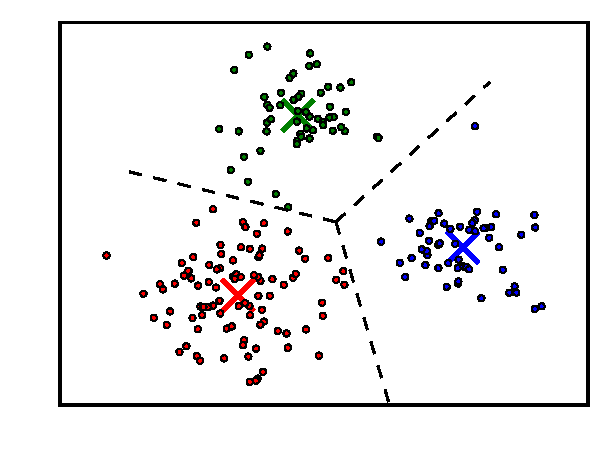
\includegraphics[width=0.7\textwidth]{kmeans-10}}%
  \end{center}
\end{frame}

%\begin{frame}{Clustering: $K$-means algorithm}
%\end{frame}


\end{document}

